\documentclass[11pt,a4paper]{article}
\usepackage[T1]{fontenc}
\usepackage[utf8]{inputenc}
\usepackage{mathpazo}
\usepackage[margin=2.4cm]{geometry}
\usepackage{amsmath,amssymb,bm}
\usepackage{graphicx,booktabs,array,xcolor}
\usepackage[most]{tcolorbox}
\usepackage{tikz}
\usetikzlibrary{arrows.meta,positioning}
\usepackage{enumitem}
\usepackage[hidelinks]{hyperref}
\usepackage[style=numeric,sorting=none,maxbibnames=4,giveninits=true,doi=true,url=false]{biblatex}
\DeclareSourcemap{\maps[datatype=bibtex]{\map{\step[fieldset=note,null]}}}
\addbibresource{refs.bib}
\setlength{\parindent}{0pt}
\setlength{\parskip}{6pt}
\setlist{itemsep=2pt,topsep=3pt}

% generated by figures.py, do not edit
\newcommand{\npApLAD}{0.243}
\newcommand{\npAmLAD}{0.095}
\newcommand{\npAdLAD}{0.031}
\newcommand{\npApLCx}{0.090}
\newcommand{\npAmLCx}{0.045}
\newcommand{\npAdLCx}{0.017}
\newcommand{\npApRCA}{0.085}
\newcommand{\npAmRCA}{0.067}
\newcommand{\npAdRCA}{0.037}
\newcommand{\npThreeNone}{0.664}
\newcommand{\npThreeAny}{0.336}
\newcommand{\nchopOne}{0.5000}
\newcommand{\nchopTwo}{0.4375}
\newcommand{\nchopTen}{0.4013}
\newcommand{\nchopHundred}{0.3942}
\newcommand{\nchopThousand}{0.3935}
\newcommand{\nchopExact}{0.3935}
\newcommand{\naddLone}{0.10}
\newcommand{\naddLtwo}{0.05}
\newcommand{\naddPone}{0.0952}
\newcommand{\naddPtwo}{0.0488}
\newcommand{\naddPsum}{0.1393}
\newcommand{\naddPprod}{0.1393}
\newcommand{\nhrBaseLow}{0.01}
\newcommand{\nhrLamLow}{0.0101}
\newcommand{\nhrNewLow}{0.0150}
\newcommand{\nhrORLow}{1.50}
\newcommand{\nhrRRLow}{1.50}
\newcommand{\nhrBaseMid}{0.10}
\newcommand{\nhrLamMid}{0.1054}
\newcommand{\nhrNewMid}{0.1462}
\newcommand{\nhrORMid}{1.54}
\newcommand{\nhrRRMid}{1.46}
\newcommand{\nhrBaseHigh}{0.50}
\newcommand{\nhrLamHigh}{0.6931}
\newcommand{\nhrNewHigh}{0.6464}
\newcommand{\nhrORHigh}{1.83}
\newcommand{\nhrRRHigh}{1.29}
\newcommand{\nlnkEtaA}{-3.0}
\newcommand{\nlnkLamA}{0.0498}
\newcommand{\nlnkPA}{0.0486}
\newcommand{\nlnkLogitA}{0.0474}
\newcommand{\nlnkEtaB}{-1.0}
\newcommand{\nlnkLamB}{0.3679}
\newcommand{\nlnkPB}{0.3078}
\newcommand{\nlnkLogitB}{0.2689}
\newcommand{\nlnkEtaC}{0.5}
\newcommand{\nlnkLamC}{1.6487}
\newcommand{\nlnkPC}{0.8077}
\newcommand{\nlnkLogitC}{0.6225}
\newcommand{\netaApLAD}{-1.28}
\newcommand{\nalphapLAD}{-2.2}
\newcommand{\npAzeropLAD}{0.243}
\newcommand{\netaAmLAD}{-2.30}
\newcommand{\nalphamLAD}{-2.6}
\newcommand{\npAzeromLAD}{0.095}
\newcommand{\netaAdLAD}{-3.47}
\newcommand{\nalphadLAD}{-3.6}
\newcommand{\npAzerodLAD}{0.031}
\newcommand{\netaApLCx}{-2.36}
\newcommand{\nalphapLCx}{-3.0}
\newcommand{\npAzeropLCx}{0.090}
\newcommand{\netaAmLCx}{-3.08}
\newcommand{\nalphamLCx}{-3.4}
\newcommand{\npAzeromLCx}{0.045}
\newcommand{\netaAdLCx}{-4.05}
\newcommand{\nalphadLCx}{-4.0}
\newcommand{\npAzerodLCx}{0.017}
\newcommand{\netaApRCA}{-2.42}
\newcommand{\nalphapRCA}{-2.8}
\newcommand{\npAzeropRCA}{0.085}
\newcommand{\netaAmRCA}{-2.67}
\newcommand{\nalphamRCA}{-3.2}
\newcommand{\npAzeromRCA}{0.067}
\newcommand{\netaAdRCA}{-3.29}
\newcommand{\nalphadRCA}{-3.6}
\newcommand{\npAzerodRCA}{0.037}
\newcommand{\ncpLADscoretwo}{+0.250}
\newcommand{\ncpLADlen}{+0.060}
\newcommand{\ncpLADcurv}{+0.240}
\newcommand{\ncpLADtaper}{+0.090}
\newcommand{\ncpLADlm}{+0.250}
\newcommand{\ncpLADrlad}{+0.030}
\newcommand{\ncpLADrlcx}{+0.000}
\newcommand{\nxpLADscoretwo}{+0.5}
\newcommand{\nxpLADlen}{+0.1}
\newcommand{\nxpLADcurv}{+1.2}
\newcommand{\nxpLADtaper}{+0.6}
\newcommand{\nxpLADlm}{+1.0}
\newcommand{\nxpLADrlad}{+0.3}
\newcommand{\nxpLADrlcx}{+0.0}
\newcommand{\nLampLAD}{0.2780}
\newcommand{\nzmupLAD}{0.08}
\newcommand{\nzsdpLAD}{0.02}
\newcommand{\nzmudRCA}{0.12}
\newcommand{\nzsddRCA}{0.04}
\newcommand{\nzxpLAD}{0.11}
\newcommand{\nzzpLAD}{1.5}
\newcommand{\nzxdRCA}{0.11}
\newcommand{\nzzdRCA}{-0.25}
\newcommand{\nrawpLAD}{0.10}
\newcommand{\nrawdRCA}{0.05}
\newcommand{\nrawHRpLAD}{1.105}
\newcommand{\nrawHRdRCA}{1.051}
\newcommand{\nbetascoretwo}{0.50}
\newcommand{\nHRscoretwo}{1.649}
\newcommand{\nbetalen}{0.60}
\newcommand{\nHRlen}{1.822}
\newcommand{\nbetacurv}{0.20}
\newcommand{\nHRcurv}{1.221}
\newcommand{\nbetataper}{0.15}
\newcommand{\nHRtaper}{1.162}
\newcommand{\nbetalm}{0.25}
\newcommand{\nHRlm}{1.284}
\newcommand{\nbetarlad}{0.10}
\newcommand{\nHRrlad}{1.105}
\newcommand{\nbetarlcx}{0.10}
\newcommand{\nHRrlcx}{1.105}
\newcommand{\nsigma}{1.1}
\newcommand{\nsigmasq}{1.21}
\newcommand{\nMHR}{2.86}
\newcommand{\nfrailMinus}{0.368}
\newcommand{\nfrailZero}{1.000}
\newcommand{\nfrailPlus}{2.718}
\newcommand{\nfrailLo}{0.33}
\newcommand{\nfrailHi}{3.00}
\newcommand{\nfrailOut}{0.32}
\newcommand{\npApLADbPlus}{0.530}
\newcommand{\npApLADbMinus}{0.097}
\newcommand{\ncorrBoth}{0.0266}
\newcommand{\ncorrProd}{0.0135}
\newcommand{\ncorrRatio}{2.0}
\newcommand{\nSA}{0.7627}
\newcommand{\nlogSA}{-0.271}
\newcommand{\nmaxEtaA}{-1.280}
\newcommand{\nPAgivenZero}{0.534}
\newcommand{\nPAgivenMinus}{0.245}
\newcommand{\nPAgivenZ}{0.534}
\newcommand{\nPAgivenPlus}{0.874}
\newcommand{\nghxA}{-2.020}
\newcommand{\nghwA}{0.0200}
\newcommand{\nghbA}{-3.143}
\newcommand{\nghfA}{0.0324}
\newcommand{\nghwnA}{0.0113}
\newcommand{\nghcA}{0.0004}
\newcommand{\nghxB}{-0.959}
\newcommand{\nghwB}{0.3936}
\newcommand{\nghbB}{-1.491}
\newcommand{\nghfB}{0.1578}
\newcommand{\nghwnB}{0.2221}
\newcommand{\nghcB}{0.0350}
\newcommand{\nghxC}{+0.000}
\newcommand{\nghwC}{0.9453}
\newcommand{\nghbC}{+0.000}
\newcommand{\nghfC}{0.5336}
\newcommand{\nghwnC}{0.5333}
\newcommand{\nghcC}{0.2846}
\newcommand{\nghxD}{+0.959}
\newcommand{\nghwD}{0.3936}
\newcommand{\nghbD}{+1.491}
\newcommand{\nghfD}{0.9662}
\newcommand{\nghwnD}{0.2221}
\newcommand{\nghcD}{0.2146}
\newcommand{\nghxE}{+2.020}
\newcommand{\nghwE}{0.0200}
\newcommand{\nghbE}{+3.143}
\newcommand{\nghfE}{1.0000}
\newcommand{\nghwnE}{0.0113}
\newcommand{\nghcE}{0.0113}
\newcommand{\nPAfive}{0.5458}
\newcommand{\nPAforty}{0.5476}
\newcommand{\nPAtwohundred}{0.5476}
\newcommand{\nPAtrue}{0.548}
\newcommand{\nPAbzero}{0.534}
\newcommand{\nPAnaive}{0.687}
\newcommand{\nPBtrue}{0.291}
\newcommand{\nPBbzero}{0.222}
\newcommand{\nPBnaive}{0.352}
\newcommand{\nSB}{0.2516}
\newcommand{\nPCtrue}{0.667}
\newcommand{\nPCbzero}{0.710}
\newcommand{\nPCnaive}{0.833}
\newcommand{\nSC}{1.2387}
\newcommand{\nmApLAD}{0.311}
\newcommand{\nmAmLAD}{0.146}
\newcommand{\nmAdLAD}{0.052}
\newcommand{\nmApLCx}{0.139}
\newcommand{\nmAmLCx}{0.075}
\newcommand{\nmAdLCx}{0.030}
\newcommand{\nmApRCA}{0.132}
\newcommand{\nmAmRCA}{0.108}
\newcommand{\nmAdRCA}{0.062}
\newcommand{\ncoinLOne}{0.000478}
\newcommand{\ncoinLLOne}{-7.65}
\newcommand{\ncoinLThree}{0.002224}
\newcommand{\ncoinLLThree}{-6.11}
\newcommand{\ncoinLFive}{0.000977}
\newcommand{\ncoinLLFive}{-6.93}
\newcommand{\ntoyN}{600}
\newcommand{\ntoyRows}{5,400}
\newcommand{\ntoySegEvents}{492}
\newcommand{\ntoyPersonEvents}{267}
\newcommand{\ntoyPersonPct}{44}
\newcommand{\nllFull}{-1414.06}
\newcommand{\nllBase}{-1441.28}
\newcommand{\nLR}{54.44}
\newcommand{\nLRdf}{5}
\newcommand{\nLRp}{1.7\times 10^{-10}}
\newcommand{\nchiCrit}{11.07}
\newcommand{\nestscoretwo}{0.50}
\newcommand{\nestHRscoretwo}{1.64}
\newcommand{\nestlen}{0.87}
\newcommand{\nestHRlen}{2.38}
\newcommand{\nestcurv}{0.25}
\newcommand{\nestHRcurv}{1.28}
\newcommand{\nesttaper}{0.18}
\newcommand{\nestHRtaper}{1.20}
\newcommand{\nestlm}{0.26}
\newcommand{\nestHRlm}{1.29}
\newcommand{\nestrlad}{0.15}
\newcommand{\nestHRrlad}{1.16}
\newcommand{\nestrlcx}{0.20}
\newcommand{\nestHRrlcx}{1.22}
\newcommand{\nestsigma}{1.08}
\newcommand{\nestsigmaBase}{1.07}
\newcommand{\ngammaShape}{0.425}
\newcommand{\ngammaScale}{4.310}
\newcommand{\nPAgamma}{0.461}


\definecolor{cIdea}{HTML}{2a6fb0}
\definecolor{cEx}{HTML}{3a9a5b}
\definecolor{cWhy}{HTML}{e07b1a}
\definecolor{cRecap}{HTML}{7b4fa8}
\definecolor{cWarn}{HTML}{c23b3b}
\newtcolorbox{idea}[1][]{colback=cIdea!6,colframe=cIdea,fonttitle=\bfseries,title=Idea,#1}
\newtcolorbox{example}[1][]{colback=cEx!6,colframe=cEx,fonttitle=\bfseries,title=Worked example,#1}
\newtcolorbox{why}[1][]{colback=cWhy!6,colframe=cWhy,fonttitle=\bfseries,title=Why the model needs this,#1}
\newtcolorbox{recap}[1][]{colback=cRecap!6,colframe=cRecap,fonttitle=\bfseries,title=Recap,#1}
\newtcolorbox{caution}[1][]{colback=cWarn!5,colframe=cWarn,fonttitle=\bfseries,title=Careful,#1}
\newcommand{\fig}[3][0.95]{\begin{center}\includegraphics[width=#1\linewidth]{fig/#2}\\[-2pt]{\small #3}\end{center}}
\newcommand{\e}{\mathrm{e}}

\title{The pooled cloglog model, step by step\\[4pt]
\large From one coin flip to a person's risk of developing coronary plaque}
\author{Learning notes for the CGPS (Herlev--Østerbro) who analysis}
\date{3 November 2026}

\begin{document}
\maketitle

\begin{tcolorbox}[colback=black!3,colframe=black!40,title=How to read this]
Every step adds one new piece of maths. Each piece comes with a picture and a small example with real numbers.
All numbers are made up: three toy people, \textbf{A}, \textbf{B} and \textbf{C}, each with the nine trunk segments
(proximal, mid and distal LAD, LCx and RCA), and one simulated toy cohort of \ntoyN{} people.
No CGPS data appear anywhere. The numbers are computed by \texttt{figures.py} with the same formulas as
\texttt{CGPS\_data/progression\_who\_pooled.py}, so the text, the figures and the code agree.

Section~\ref{sec:full} puts the whole model on one page. Come back to it whenever you lose track.
The covariates follow the \emph{planned} design (SCORE2, segment position, log length, curvature, taper, the LM angle and
the two LM diameter ratios). The box in Section~\ref{sec:full} lists where the current code differs.
\end{tcolorbox}

\tableofcontents
\newpage

%=====================================================================
\section{Probability and a yes/no outcome}
\label{sec:prob}

\begin{idea}
A \textbf{probability} is a number between 0 and 1 that says how often something happens in the long run.
$p = 0.25$ means: among many people exactly like this one, about one in four.
\end{idea}

For every person $i$ and every segment $j$ the outcome is a yes/no answer: did plaque appear in this segment between the
baseline scan and the follow-up scan about ten years later? Write it as a number,
\[
y_{ij} = \begin{cases} 1 & \text{plaque at follow-up (``yes'')} \\ 0 & \text{no plaque (``no'')} \end{cases}
\]
The subscripts are labels: $i$ says \emph{which person}, $j$ says \emph{which segment}. $y_{\text{A},\text{pLAD}}$ is the
outcome of person A's proximal LAD.

A yes/no outcome with probability $p$ of ``yes'' is called a \textbf{Bernoulli trial}: a coin that lands ``yes'' with
probability $p$ and ``no'' with probability $1-p$. Each segment is its own coin, with its own $p_{ij}$.

\fig[0.8]{f01_tree_p}{Figure 1. Person A's nine coins. Each number is the chance that the segment develops plaque within
ten years (for now with the person effect $b$ of Section~\ref{sec:frailty} set to zero).}

\begin{example}
Person A's pLAD has $p = \npApLAD$. Among 1{,}000 people exactly like A, about $243$ would develop plaque in the pLAD.
The chance of ``no'' is $1 - \npApLAD = 0.757$.
\end{example}

One formula covers both answers, and it is used again for fitting in Section~\ref{sec:lik}:
\[
P(y) = p^{\,y}\,(1-p)^{1-y}.
\]
For $y=1$ it gives $p^1 (1-p)^0 = p$; for $y = 0$ it gives $p^0 (1-p)^1 = 1-p$ (any number to the power 0 is 1).

\begin{recap}
$y_{ij}\in\{0,1\}$; $p_{ij}$ = chance of $y_{ij}=1$; $P(y)=p^y(1-p)^{1-y}$.
\end{recap}

%=====================================================================
\section{Several segments, one person}
\label{sec:several}

The who question is about the \emph{person}: does A develop plaque \emph{anywhere} in the nine segments?

\begin{idea}
If two events do not influence each other (they are \textbf{independent}), the chance that both happen is the
product of their chances. ``Plaque nowhere'' means ``no'' in segment 1 \emph{and} ``no'' in segment 2 \emph{and} \ldots
\end{idea}

\fig[0.95]{f02_probtree}{Figure 2. All $2^3 = 8$ possible outcomes of A's three LAD segments. Multiply along a path to get
its probability. Only one path has no plaque at all.}

\begin{example}
For A's three LAD segments:
\[
P(\text{no plaque in the LAD}) = (1-\npApLAD)(1-\npAmLAD)(1-\npAdLAD) = \npThreeNone,
\]
so $P(\text{plaque somewhere in the LAD}) = 1 - \npThreeNone = \npThreeAny$.
It is easier to compute ``none'' and subtract from 1 than to add up the seven paths with at least one P.
\end{example}

The capital Greek letter $\Pi$ (``pi'') is shorthand for ``multiply all of these'':
\[
P(\text{no plaque in any segment}) = \prod_{j=1}^{9}(1-p_{ij}),\qquad
P(\text{any plaque}) = 1-\prod_{j=1}^{9}(1-p_{ij}).
\]

\begin{caution}
This product assumes the segments are independent. In real people they are not: someone whose pLAD develops plaque is
more likely to develop it elsewhere too. Section~\ref{sec:corr} shows how the model repairs this, and
Section~\ref{sec:shortcuts} shows what goes wrong if you ignore it.
\end{caution}

%=====================================================================
\section{Rates, hazards and the exponential function}
\label{sec:hazard}

Plaque does not appear at the moment of the follow-up scan. It starts at some point during the ten years. The model
describes this with a \textbf{hazard}: the rate at which plaque starts.

\begin{idea}
Chop the ten years into $n$ short pieces. In each piece, plaque starts with a small chance. The total of these small chances
over the window is the \textbf{cumulative hazard} $\Lambda$ (capital ``lambda''). With $n$ pieces of chance $\Lambda/n$
each, the chance that plaque never starts is $(1-\Lambda/n)^n$.
\end{idea}

\begin{example}
Take $\Lambda = 0.5$. The chance that plaque \emph{does} start at some point, $1-(1-0.5/n)^n$:

\begin{center}
\begin{tabular}{lcccccc}
\toprule
pieces $n$ & 1 & 2 & 10 & 100 & 1000 & infinitely many\\
P(onset) & \nchopOne & \nchopTwo & \nchopTen & \nchopHundred & \nchopThousand & \nchopExact\\
\bottomrule
\end{tabular}
\end{center}
As the pieces get finer, the answer settles on $1-\e^{-0.5} = \nchopExact$.
\end{example}

This limit is where the number $\e \approx 2.718$ comes from. The rule is
\[
\boxed{\;p = 1-\e^{-\Lambda}\;}
\]
$\e^{x}$, also written $\exp(x)$, is the \textbf{exponential function}. Its partner is the \textbf{natural logarithm}
$\log$, which undoes it: $\log(\e^{x}) = x$ and $\e^{\log u} = u$.

\fig{f04_exp_log}{Figure 3. Left: $\e^x$ turns any number, also a negative one, into a positive one. Right: $\log$ goes
back. $\log 1 = 0$, numbers below 1 have a negative log.}

Three rules are used again and again below:
\[
\e^{a}\,\e^{b} = \e^{a+b},\qquad \log(a\cdot b) = \log a + \log b,\qquad \e^{0}=1.
\]

\fig{f03_hazard_to_p}{Figure 4. Left: chopping the window finer converges to $1-\e^{-\Lambda}$. Right: the curve
$p = 1-\e^{-\Lambda}$. For small $\Lambda$, $p\approx\Lambda$; for large $\Lambda$, $p$ flattens below 1.}

\begin{why}
A probability is stuck between 0 and 1, a hazard is not: it can be any positive number. Hazards can be multiplied by a
risk factor without ever producing an impossible probability. One way to picture $\Lambda$: if plaque could start more than
once, $\Lambda$ is the expected number of starts in the window, and $p$ is the chance of at least one (a Poisson process;
\cite{statacorp2025mecloglog}).
\end{why}

%=====================================================================
\section{Hazards add up}
\label{sec:add}

\begin{idea}
The chance of no plaque in two segments is $\e^{-\Lambda_1}\cdot\e^{-\Lambda_2} = \e^{-(\Lambda_1+\Lambda_2)}$. So two
segments together behave like one segment whose hazard is the \textbf{sum} of the two.
\end{idea}

\fig{f05_hazards_add}{Figure 5. Adding hazards and multiplying ``no'' probabilities give the same person risk.}

\begin{example}
Segment 1: $\Lambda_1 = \naddLone$, so $p_1 = 1-\e^{-0.10} = \naddPone$.
Segment 2: $\Lambda_2 = \naddLtwo$, so $p_2 = \naddPtwo$.
\begin{itemize}
\item Route 1, add hazards: $1-\e^{-(0.10+0.05)} = \naddPsum$.
\item Route 2, multiply ``no'': $1-(1-\naddPone)(1-\naddPtwo) = \naddPprod$.
\end{itemize}
\end{example}

The capital Greek letter $\Sigma$ (``sigma'') means ``add all of these''. For person $i$, the \textbf{sum of the segment
hazards} gets its own name:
\[
S_i = \sum_{j=1}^{9}\Lambda_{ij},\qquad P(\text{any plaque}) = 1-\e^{-S_i}.
\]

\begin{why}
$S_i$ is the bridge from segments to the person. Section~\ref{sec:given} shows that the person risk depends on the nine
segments only through this one number.
\end{why}

%=====================================================================
\section{Proportional hazards and the hazard ratio}
\label{sec:ph}

\begin{idea}
A risk factor \textbf{multiplies} the hazard. If a segment has hazard ratio (HR) 1.5, its hazard is 1.5 times the hazard of an
otherwise identical reference segment: $\Lambda = \Lambda_0 \times \text{HR}$. The ratio is the same whatever $\Lambda_0$ is.
This is the \textbf{proportional hazards} assumption.
\end{idea}

\begin{example}
HR $=1.5$ at three baseline risks. ``RR'' is the risk ratio $p_\text{new}/p_\text{ref}$; the odds ratio (OR) compares
odds $p/(1-p)$.
\begin{center}
\begin{tabular}{ccccc}
\toprule
$p_\text{ref}$ & $\Lambda_0 = -\log(1-p_\text{ref})$ & $p_\text{new}=1-\e^{-1.5\Lambda_0}$ & RR & OR\\
\midrule
\nhrBaseLow & \nhrLamLow & \nhrNewLow & \nhrRRLow & \nhrORLow\\
\nhrBaseMid & \nhrLamMid & \nhrNewMid & \nhrRRMid & \nhrORMid\\
\nhrBaseHigh & \nhrLamHigh & \nhrNewHigh & \nhrRRHigh & \nhrORHigh\\
\bottomrule
\end{tabular}
\end{center}
The hazard ratio is 1.5 in every row. The risk ratio and the odds ratio drift with the baseline risk.
\end{example}

\fig{f06_hr_vs_or}{Figure 6. One and the same risk factor (HR $=1.5$) reads as different odds ratios and risk ratios
depending on how common plaque already is.}

\begin{why}
The nine segments have very different baseline risks (the pLAD is far more prone than the dLCx). A hazard ratio lets one
coefficient mean the same thing in all nine. This model, for an event known only to have happened within an interval, is
the grouped-data proportional hazards model of Prentice and Gloeckler \cite{prentice1978grouped}.
\end{why}

%=====================================================================
\section{The cloglog link: from a line to a probability}
\label{sec:link}

The model has to turn a sum of terms (any number, negative or positive) into a probability. It does so in two steps.

\begin{idea}
\begin{enumerate}
\item Call the sum of terms $\eta$ (``eta''), the \textbf{linear predictor}. Make the hazard $\Lambda = \e^{\eta}$, which is
always positive.
\item Make the probability $p = 1-\e^{-\Lambda}$ (Section~\ref{sec:hazard}).
\end{enumerate}
Together: $p = 1-\exp\!\left(-\e^{\eta}\right)$. Undoing both steps gives $\eta = \log\{-\log(1-p)\}$, the
\textbf{complementary log-log}, or \textbf{cloglog}, of $p$.
\end{idea}

\begin{example}
\begin{center}
\begin{tabular}{cccc}
\toprule
$\eta$ & $\Lambda=\e^{\eta}$ & cloglog $p = 1-\e^{-\Lambda}$ & logit $p = 1/(1+\e^{-\eta})$\\
\midrule
\nlnkEtaA & \nlnkLamA & \nlnkPA & \nlnkLogitA\\
\nlnkEtaB & \nlnkLamB & \nlnkPB & \nlnkLogitB\\
\nlnkEtaC & \nlnkLamC & \nlnkPC & \nlnkLogitC\\
\bottomrule
\end{tabular}
\end{center}
At low risk ($\eta = -3$) cloglog and logit hardly differ. They separate at higher risk.
\end{example}

\fig{f07_link}{Figure 7. The cloglog curve and the more familiar logit curve. At low risk they nearly coincide.}

\begin{why}
The log turns ``multiply the hazard'' into ``add to $\eta$'': $\log(\Lambda_0\cdot\text{HR}) = \log\Lambda_0 + \log\text{HR}$.
So a coefficient $\beta$ added to $\eta$ multiplies the hazard by $\e^{\beta}$: \textbf{$\e^{\beta}$ is a hazard ratio}.
With the logit link, $\e^{\beta}$ would be an odds ratio, which drifts with the baseline risk (Figure~6). The cloglog link is
the usual choice for rare binary outcomes and for this hazard reading \cite{statacorp2025mecloglog,prentice1978grouped}.
\end{why}

%=====================================================================
\section{The linear predictor: adding up the terms}
\label{sec:eta}

\begin{idea}
$\eta_{ij}$ is a weighted sum. Each covariate value $x$ is multiplied by its coefficient $\beta$ (``beta''), and the
results are added to a starting value $\alpha_j$ (``alpha'') for the segment type:
\[
\eta_{ij} = \alpha_j + \beta_1 x_{ij,1} + \beta_2 x_{ij,2} + \dots
\]
\end{idea}

The terms in the planned model:
\begin{itemize}
\item $\alpha_j$: one value per segment type (nine in total). It is the log hazard of that segment for a reference person
with all covariates at 0. It carries ``plaque is more common proximally and in the LAD''.
\item SCORE2 (z-scored, Section~\ref{sec:z}): the same value on all nine rows of a person.
\item log length: longer segments have more wall where plaque can start. If its coefficient were exactly 1, hazard would be
proportional to length; the model estimates it freely.
\item curvature and taper (z within segment type): a different value on every row.
\item the LM angle and the LM$\to$LAD and LM$\to$LCx diameter ratios: one value per person, entered only on the rows they
can act on (Section~\ref{sec:geom}).
\end{itemize}

In the toy model the coefficients are $\beta_\text{SCORE2}=\nbetascoretwo$, $\beta_\text{length}=\nbetalen$,
$\beta_\text{curv}=\nbetacurv$, $\beta_\text{taper}=\nbetataper$, $\beta_\text{LM angle}=\nbetalm$ and
$\beta_\text{LM$\to$LAD}=\beta_\text{LM$\to$LCx}=\nbetarlad$.

\begin{example}[title={Worked example: Person A's pLAD}]
\begin{center}
\begin{tabular}{lrrr}
\toprule
term & value $x$ & coefficient $\beta$ & $\beta\cdot x$\\
\midrule
$\alpha_\text{pLAD}$ & & & $\nalphapLAD$\\
SCORE2 (z) & \nxpLADscoretwo & \nbetascoretwo & \ncpLADscoretwo\\
log length & \nxpLADlen & \nbetalen & \ncpLADlen\\
curvature (z) & \nxpLADcurv & \nbetacurv & \ncpLADcurv\\
taper (z) & \nxpLADtaper & \nbetataper & \ncpLADtaper\\
LM angle (z) & \nxpLADlm & \nbetalm & \ncpLADlm\\
LM$\to$LAD ratio (z) & \nxpLADrlad & \nbetarlad & \ncpLADrlad\\
LM$\to$LCx ratio (z) & off on LAD rows & \nbetarlcx & $0$\\
\midrule
$\eta_{\text{A},\text{pLAD}}$ & & & $\netaApLAD$\\
\bottomrule
\end{tabular}
\end{center}
Hazard: $\Lambda = \e^{\netaApLAD} = \nLampLAD$. Probability: $p = 1-\e^{-\nLampLAD} = \npApLAD$.
\end{example}

\fig{f08_eta_bars}{Figure 8. Left: the same calculation as a waterfall. Each bar moves $\eta$ up or down from $\alpha_\text{pLAD}$.
Right: the probabilities of all nine of A's segments.}

\begin{recap}
Compact notation: stack the covariates in a list (a \textbf{vector}) $\mathbf{x}_{ij}$ and the coefficients in
$\bm\beta$. Then $\eta_{ij} = \alpha_j + \mathbf{x}_{ij}^\top\bm\beta$, where $\mathbf{x}^\top\bm\beta$ means ``multiply
pairwise and add''. Reading a coefficient: one unit more of $x$ multiplies the segment hazard by $\e^{\beta}$. For SCORE2
that is $\e^{\nbetascoretwo} = \nHRscoretwo$ per SD.
\end{recap}

%=====================================================================
\section{z-scores within segment type}
\label{sec:z}

Curvature means different things in different segments. Distal segments bend more than proximal ones, so ``0.11 per mm''
is a lot in the pLAD and ordinary in the dRCA.

\begin{idea}
A \textbf{z-score} says how many standard deviations (SD) a value lies above or below the average:
\[
z_{ij} = \frac{x_{ij} - m_j}{s_j},
\]
where $m_j$ and $s_j$ are the mean and SD of $x$ \emph{in segment type $j$}. The SD measures the typical spread around
the mean.
\end{idea}

\fig{f09_zscore}{Figure 9. Made-up curvature distributions for the pLAD and the dRCA. The red line marks $z=+1$ in each.}

\begin{example}
A curvature of $\nzxpLAD$ per mm:
\begin{itemize}
\item in a pLAD (mean $\nzmupLAD$, SD $\nzsdpLAD$): $z = (0.11-0.08)/0.02 = \nzzpLAD$, a strongly bent pLAD;
\item in a dRCA (mean $\nzmudRCA$, SD $\nzsddRCA$): $z = (0.11-0.12)/0.04 = \nzzdRCA$, a slightly straighter than usual dRCA.
\end{itemize}
\end{example}

\begin{why}
One shared coefficient on $z$ means: ``1 SD more curved than usual \emph{for this segment type}'' carries the same hazard
ratio everywhere. In raw units the effect differs by segment: the hazard ratio per $0.01$ per mm is
$\exp(\beta\cdot 0.01/s_j)$, that is $\exp(\nrawpLAD) = \nrawHRpLAD$ in the pLAD and $\exp(\nrawdRCA) = \nrawHRdRCA$ in
the dRCA. Segment types with a narrow spread get a steeper raw slope. The mean $m_j$ is absorbed by $\alpha_j$ anyway; the
scaling by $s_j$ is the real choice.
\end{why}

\begin{caution}
$m_j$ and $s_j$ must come from the people the model is trained on. In cross-validation they are recomputed in every
training fold.
\end{caution}

%=====================================================================
\section{The geometry terms}
\label{sec:geom}

\fig[0.82]{f10_design}{Figure 10. Person A's nine rows. Every row gets SCORE2, log length, curvature and taper. The LM angle
sits only on the pLAD and pLCx rows, the LM$\to$LAD ratio only on LAD rows, the LM$\to$LCx ratio only on LCx rows. A grey
0 switches the term off on that row.}

\begin{idea}
Curvature and taper are measured per segment, so they enter every row. The LM bifurcation features are measured once per
person and enter only on the rows downstream of the bifurcation they describe. Putting 0 on the other rows fixes their
coefficient there at zero, which costs no extra parameter.
\end{idea}

\begin{example}
The per-SD hazard ratios of the toy model:
curvature $\e^{\nbetacurv} = \nHRcurv$, taper $\e^{\nbetataper} = \nHRtaper$, LM angle $\e^{\nbetalm} = \nHRlm$, each
diameter ratio $\e^{\nbetarlad} = \nHRrlad$.
A pLAD that is 1 SD more curved than usual has $\nHRcurv$ times the hazard of an otherwise identical pLAD of the same person.
\end{example}

\fig{f11_shared_vs_artery}{Figure 11. Left: the primary model, one slope for all arteries. Right: the planned secondary
test, one slope per artery for curvature and taper (two extra slopes each, 4 extra parameters).}

\begin{why}
The five geometry terms together form the \textbf{geometry block} (5 parameters). The one prespecified test of the who
question asks whether this block improves the model (Section~\ref{sec:lr}). Whether geometry acts differently by artery is a
separate, secondary test, so it cannot change the primary answer.
\end{why}

%=====================================================================
\section{People differ: the random intercept}
\label{sec:frailty}

Two people with the same SCORE2 and the same geometry can still differ in risk: genes, diet and many things nobody measured.
The model gives every person an extra term $b_i$:
\[
\eta_{ij} = \alpha_j + \mathbf{x}_{ij}^\top\bm\beta + b_i.
\]

\begin{idea}
$b_i$ is unknown, so the model does not estimate it person by person. It assumes the $b_i$ are spread like a
\textbf{normal distribution} (the bell curve) with mean 0 and SD $\sigma$, written $b_i\sim N(0,\sigma^2)$. Only $\sigma$ is
estimated. About 68\% of people lie within $\pm\sigma$ of 0, about 95\% within $\pm2\sigma$.
\end{idea}

\fig{f12_normal}{Figure 12. Left: the spread of person effects in the toy model, $\sigma=\nsigma$. Right: the same spread
as a multiplier $\e^{b}$ on the hazard, called the \textbf{frailty}.}

Since $\e^{\eta+b} = \e^{\eta}\cdot\e^{b}$, the person effect multiplies \emph{all nine} hazards of a person by the same
factor $\e^{b_i}$. In survival analysis this is a \textbf{shared frailty} \cite{duchateau2008frailty}.

\begin{example}
$b = +1$ multiplies every hazard by $\e^{1} = \nfrailPlus$; $b=-1$ by $\e^{-1} = \nfrailMinus$.
For A's pLAD: $p = \npApLADbMinus$ at $b=-1$, $\npApLAD$ at $b=0$, $\npApLADbPlus$ at $b=+1$.
With $\sigma = \nsigma$, the middle 68\% of people have frailties between $\e^{-1.1}=\nfrailLo$ and $\e^{1.1}=\nfrailHi$.
\end{example}

\fig{f13_frailty_shift}{Figure 13. The same geometry, three values of the unmeasured person effect.}

\begin{why}
$\sigma$ is hard to picture. The \textbf{median hazard ratio} translates it: pick two random people with identical
covariates and divide the higher hazard by the lower; the median of that ratio is
$\text{MHR} = \exp\!\big(\sqrt{2\sigma^2}\times 0.6745\big) = \nMHR$ for $\sigma=\nsigma$ \cite{austin2017mhr}.
(0.6745 is the point that cuts off the upper quarter of a standard bell curve.)
\end{why}

%=====================================================================
\section{Why segments of one person go together}
\label{sec:corr}

\begin{idea}
Given $b_i$, the nine coins of person $i$ are independent. But $b_i$ is shared. If one segment of a person developed plaque,
that hints that $b_i$ is high, which raises the chance for the others. Without knowing $b_i$, the segments are
\textbf{positively correlated}.
\end{idea}

\begin{example}
Two segments with $\eta = -2.5$ each and $\sigma = 1$ (simulated with 400{,}000 people):
$P(\text{both}) = \ncorrBoth$, while $P(\text{seg 1})\times P(\text{seg 2}) = \ncorrProd$.
Both-segment plaque is about $\ncorrRatio$ times as common as independence predicts.
\end{example}

\fig[0.7]{f14_correlation}{Figure 14. The larger $\sigma$, the more plaque clusters within people. At $\sigma=0$ the two lines meet.}

\begin{why}
Treating the 5{,}400 rows of a cohort as independent would overstate how much information the data hold. One alternative,
generalized estimating equations (GEE), corrects the standard errors but gives no person risk formula
\cite{liang1986longitudinal}. The random intercept models the dependence directly, and that is what makes the next step
possible.
\end{why}

%=====================================================================
\section{From segments to a person, for a known $b$}
\label{sec:given}

Fix $b$ for a moment. Then the segments are independent, and Sections~\ref{sec:several}--\ref{sec:add} apply:
\[
P(\text{no plaque anywhere}\mid b) = \prod_{j}\exp\!\big(-\e^{\eta_{ij}+b}\big)
= \exp\!\Big(-\e^{b}\sum_j \e^{\eta_{ij}}\Big) = \exp\!\big(-\e^{b}S_i\big).
\]
The vertical bar ``$\mid b$'' reads ``given $b$''. $S_i = \sum_j \e^{\eta_{ij}}$ is the sum of the nine segment hazards at
$b=0$.

\begin{idea}
For a known $b$, ``any plaque in the person'' is itself a cloglog model, with hazard $\e^{b}S_i$. The nine segments matter
only through their summed hazard.
\end{idea}

\begin{example}
Person A: $S_\text{A} = \nSA$. The pLAD alone contributes $\nLampLAD$, about 36\% of it.
\begin{itemize}
\item $b = -1$: $1-\exp(-0.368\times\nSA) = \nPAgivenMinus$
\item $b = 0$: $1-\exp(-\nSA) = \nPAgivenZ$
\item $b = +1$: $1-\exp(-2.718\times\nSA) = \nPAgivenPlus$
\end{itemize}
\end{example}

\begin{why}
The share explains why local geometry moves person risk only a little. If the pLAD had a segment HR of 1.3, A's summed
hazard would grow by a factor $(1-0.36) + 0.36\times1.3 \approx 1.11$, not 1.3. Person-level gains from segment geometry
are diluted by the segments it does not touch.
\end{why}

%=====================================================================
\section{Averaging over the unknown $b$: an integral}
\label{sec:integral}

For a new person, $b$ is unknown. The person risk is the average of $P(\text{any}\mid b)$ over all possible $b$, each
weighted by how common it is:
\[
\boxed{\;P_i = 1-\int \exp\!\big(-\e^{b}S_i\big)\,\phi(b;0,\sigma^2)\,\mathrm{d}b\;}
\]
$\phi(b;0,\sigma^2)$ is the height of the bell curve at $b$.

\begin{idea}
An \textbf{integral} $\int f(b)\,\mathrm{d}b$ is the area under a curve. Picture it as many thin bars of width
$\mathrm{d}b$ and height $f(b)$, added up. Here it is a weighted average: likely values of $b$ count a lot, rare ones a little.
\end{idea}

The integral has no formula you can write down, so it is computed numerically. \textbf{Gauss--Hermite quadrature} replaces
the curve by a handful of well-chosen points $b_k$ with weights $w_k$ \cite{liu1994gausshermite}:
\[
P_i \approx \sum_{k} \tilde w_k \,P(\text{any}\mid b_k),\qquad b_k = \sqrt2\,\sigma\,x_k,\quad \tilde w_k = w_k/\sqrt\pi ,
\]
where $x_k$ and $w_k$ are fixed numbers from a table. The $\tilde w_k$ add up to 1.

\fig{f15_integral}{Figure 15. Left: A's risk for every possible $b$. Right: the five Gauss--Hermite points. Each
weight (outline) times the risk at that point (filled) gives one purple bar; their sum is the person risk.}

\begin{example}[title={Worked example: Person A with 5 points ($\sigma=\nsigma$)}]
\begin{center}
\begin{tabular}{rrrrrr}
\toprule
$k$ & $x_k$ & $b_k=\sqrt2\sigma x_k$ & $\tilde w_k$ & $P(\text{any}\mid b_k)$ & $\tilde w_k\times P$\\
\midrule
1 & \nghxA & \nghbA & \nghwnA & \nghfA & \nghcA\\
2 & \nghxB & \nghbB & \nghwnB & \nghfB & \nghcB\\
3 & \nghxC & \nghbC & \nghwnC & \nghfC & \nghcC\\
4 & \nghxD & \nghbD & \nghwnD & \nghfD & \nghcD\\
5 & \nghxE & \nghbE & \nghwnE & \nghfE & \nghcE\\
\midrule
 & & & 1.0000 & sum & \nPAfive\\
\bottomrule
\end{tabular}
\end{center}
With 40 points: $P_\text{A} = \nPAforty$; with 200 points: $\nPAtwohundred$. Five points already land close; the code uses 40.
\end{example}

\begin{recap}
Person risk = average over the unknown person effect of the risk given that effect. It is exact under the model
\cite{duchateau2008frailty}; the only approximation is the number of quadrature points, which is checked.
\end{recap}

%=====================================================================
\section{Two tempting shortcuts, and why both fail}
\label{sec:shortcuts}

\begin{idea}
\textbf{Shortcut 1: set $b = 0$.} Zero is the \emph{median} person effect, so this gives the median person's risk, not the
average risk \cite{pavlou2015marginal}.

\textbf{Shortcut 2: multiply marginal segment risks.} First average each segment over $b$ separately, then combine them as
if independent: $1-\prod_j(1-\bar p_{ij})$. This forgets that the segments share $b$ (Section~\ref{sec:corr}).
\end{idea}

\fig[0.78]{f16_shortcuts}{Figure 16. The correct person risk (green) and the two shortcuts for the three toy people.}

\begin{example}
\begin{center}
\begin{tabular}{lcccc}
\toprule
 & $S_i$ & correct $P_i$ & $b=0$ & naive product\\
\midrule
Person A & \nSA & \nPAtrue & \nPAbzero & \nPAnaive\\
Person B & \nSB & \nPBtrue & \nPBbzero & \nPBnaive\\
Person C & \nSC & \nPCtrue & \nPCbzero & \nPCnaive\\
\bottomrule
\end{tabular}
\end{center}
A's marginal pLAD risk is $\bar p = \nmApLAD$, higher than $\npApLAD$ at $b=0$: averaging over $b$ lifts every segment, and
the product then counts the shared part of that lift nine times.
\end{example}

\begin{why}
The naive product is \emph{always} too high, for every person. Setting $b=0$ is too low for low-risk people (A, B) and too
high for high-risk ones (C); roughly, the switch happens near 0.63. Discrimination (who is ranked above whom) does not
detect the $b=0$ error, only calibration does. New people must be predicted by integrating over $b$
\cite{pavlou2015marginal,skrondal2009prediction}.
\end{why}

%=====================================================================
\section{Fitting the model: the likelihood}
\label{sec:lik}

So far the coefficients were given. In practice they are estimated from data.

\begin{idea}
The \textbf{likelihood} of a candidate value is the probability of the data you actually saw, if that value were true.
The best estimate is the value with the highest likelihood (\textbf{maximum likelihood}).
\end{idea}

\begin{example}[title={Worked example: one coin}]
10 segments, 3 with plaque. For a candidate $p$, the probability of this result is $L(p) = p^3(1-p)^7$
(Section~\ref{sec:prob}, multiplied over the 10 coins).
\begin{center}
\begin{tabular}{cccc}
\toprule
candidate $p$ & 0.1 & 0.3 & 0.5\\
$L(p)$ & \ncoinLOne & \ncoinLThree & \ncoinLFive\\
$\log L(p)$ & \ncoinLLOne & \ncoinLLThree & \ncoinLLFive\\
\bottomrule
\end{tabular}
\end{center}
$p = 0.3$ wins, which is just $3/10$.
\end{example}

\fig{f17_coin}{Figure 17. The likelihood and its log peak at the same place. Logs turn tiny products into manageable sums.}

\textbf{The full model.} For one person with a known $b$, the probability of their nine outcomes is a product over
segments. $b$ is unknown, so it is integrated out, exactly as in Section~\ref{sec:integral}:
\[
L_i(\bm\beta,\sigma) = \int \prod_{j}p_{ij}(b)^{y_{ij}}\{1-p_{ij}(b)\}^{1-y_{ij}}\,\phi(b;0,\sigma^2)\,\mathrm{d}b,
\qquad p_{ij}(b) = 1-\exp(-\e^{\eta_{ij}+b}).
\]
People are independent, so the log-likelihood of the cohort is the sum $\ell(\bm\beta,\sigma) = \sum_i \log L_i$. A computer
searches for the $(\bm\beta,\sigma)$ with the largest $\ell$, walking uphill step by step (the code uses L-BFGS-B with the
integral done by Gauss--Hermite quadrature). Quadrature centred at the mode of each person's integrand
(\emph{adaptive}) is more accurate with few points \cite{pinheiro1995approximations}; the code uses fixed points and checks
the result by doubling them.

\begin{example}[title={Worked example: the toy cohort}]
\ntoyN{} simulated people, \ntoyRows{} segment rows, \ntoySegEvents{} segments with plaque, \ntoyPersonEvents{} people
(\ntoyPersonPct\%) with plaque somewhere. Fitted against the true values:
\begin{center}
\small\setlength{\tabcolsep}{4pt}\begin{tabular}{lccccccc|c}
\toprule
 & SCORE2 & length & curv & taper & LM angle & LM$\to$LAD & LM$\to$LCx & $\sigma$\\
\midrule
true & \nbetascoretwo & \nbetalen & \nbetacurv & \nbetataper & \nbetalm & \nbetarlad & \nbetarlcx & \nsigma\\
estimate & \nestscoretwo & \nestlen & \nestcurv & \nesttaper & \nestlm & \nestrlad & \nestrlcx & \nestsigma\\
\bottomrule
\end{tabular}
\end{center}
The estimates scatter around the truth. With a different random cohort they would scatter differently; that scatter is what
standard errors and confidence intervals describe.
\end{example}

\fig{f18_likelihood}{Figure 18. Left: the log-likelihood as the curvature coefficient is moved, with everything else
re-optimized. Right: the hill over two directions at once (curvature coefficient and $\sigma$, the rest held at the peak).
The star is the maximum.}

%=====================================================================
\section{Testing geometry: the likelihood-ratio test}
\label{sec:lr}

\begin{idea}
Fit two models that differ only in the geometry block:
\begin{itemize}
\item \textbf{base}: segment intercepts, SCORE2, log length, $\sigma$;
\item \textbf{full}: base plus the 5 geometry terms.
\end{itemize}
The full model always fits at least as well. The question is whether the gain is larger than chance would give. The
\textbf{likelihood-ratio statistic} is $\text{LR} = 2(\ell_\text{full}-\ell_\text{base})$. If geometry does nothing, LR
follows a \textbf{chi-square ($\chi^2$) distribution} with degrees of freedom (df) equal to the number of added terms.
\end{idea}

\begin{example}
Toy cohort: $\ell_\text{full} = \nllFull$, $\ell_\text{base} = \nllBase$, so
$\text{LR} = 2\times(\nllFull - (\nllBase)) = \nLR$ on $\nLRdf$ df.
If geometry did nothing, LR would exceed $\nchiCrit$ only 5\% of the time. The observed LR is far beyond that:
$p = \nLRp$ (the chance of an LR this large if geometry did nothing).
\end{example}

\fig[0.8]{f19_chi2}{Figure 19. What LR looks like when geometry does nothing (blue), the top 5\% (grey) and the toy result (red).}

\begin{caution}
\begin{itemize}
\item The toy cohort was built with large geometry effects. In the real cohort the effect is expected to be small.
\item Both models must be fitted on the same rows, with the same link and the same number of quadrature points.
\item $\sigma$ is in both models, so the plain $\chi^2$ applies. Only a test of $\sigma = 0$ itself would need a different
reference distribution \cite{self1987asymptotic}.
\item The test uses both who-information (between people) and where-information (which segments within a person). A
rejection says geometry is linked to segment hazards; whether it helps rank \emph{people} is judged by the person-level
evaluation, not by this test.
\end{itemize}
\end{caution}

%=====================================================================
\section{The full model on one page}
\label{sec:full}

\begin{center}\resizebox{\linewidth}{!}{%
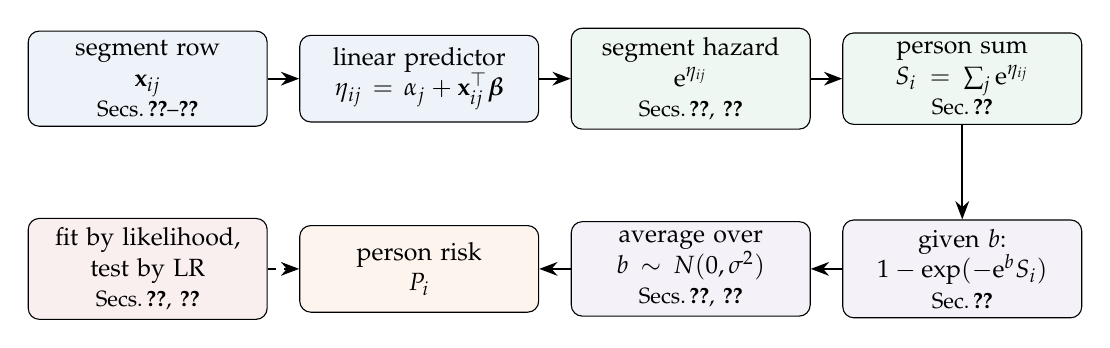
\begin{tikzpicture}[node distance=5mm and 4mm, every node/.style={font=\small},
  box/.style={draw, rounded corners, fill=#1!8, align=center, minimum height=11mm, text width=28mm,
    execute at begin node={\hyphenpenalty=10000}},
  arr/.style={-{Stealth}, thick}]
\node[box=cIdea] (x) {segment row\\$\mathbf{x}_{ij}$ \\ \footnotesize Secs.\,\ref{sec:eta}--\ref{sec:geom}};
\node[box=cIdea, right=of x] (eta) {linear predictor\\$\eta_{ij}=\alpha_j+\mathbf{x}_{ij}^\top\bm\beta$};
\node[box=cEx, right=of eta] (lam) {segment hazard\\$\e^{\eta_{ij}}$ \\ \footnotesize Secs.\,\ref{sec:hazard}, \ref{sec:link}};
\node[box=cEx, right=of lam] (S) {person sum\\$S_i=\sum_j\e^{\eta_{ij}}$ \\ \footnotesize Sec.\,\ref{sec:add}};
\node[box=cRecap, below=12mm of S] (given) {given $b$:\\$1-\exp(-\e^{b}S_i)$ \\ \footnotesize Sec.\,\ref{sec:given}};
\node[box=cRecap, left=of given] (int) {average over $b\sim N(0,\sigma^2)$ \\ \footnotesize Secs.\,\ref{sec:frailty}, \ref{sec:integral}};
\node[box=cWhy, left=of int] (P) {person risk\\$P_i$};
\node[box=cWarn, left=of P] (fit) {fit by likelihood, test by LR \\ \footnotesize Secs.\,\ref{sec:lik}, \ref{sec:lr}};
\draw[arr] (x)--(eta); \draw[arr] (eta)--(lam); \draw[arr] (lam)--(S); \draw[arr] (S)--(given);
\draw[arr] (given)--(int); \draw[arr] (int)--(P); \draw[arr,dashed] (fit)--(P);
\end{tikzpicture}}
\end{center}

\begin{tcolorbox}[colback=white,colframe=black!60,title=The model]
For person $i$ and trunk segment $j$ (pLAD, mLAD, dLAD, pLCx, mLCx, dLCx, pRCA, mRCA, dRCA):
\begin{align*}
\eta_{ij} &= \alpha_j + \beta_\text{S}\,\text{SCORE2}_i + \beta_\text{L}\log\text{length}_{ij}
  + \beta_\text{c}\,z^\text{curv}_{ij} + \beta_\text{t}\,z^\text{taper}_{ij}\\
 &\quad + \beta_\text{a}\,z^\text{LM angle}_i\,[j\in\{\text{pLAD},\text{pLCx}\}]\\
 &\quad + \beta_\text{d}\,z^\text{LM$\to$LAD}_i\,[j\in\text{LAD}] + \beta_\text{x}\,z^\text{LM$\to$LCx}_i\,[j\in\text{LCx}]\\[3pt]
P(y_{ij}=1\mid b_i) &= 1-\exp\!\big(-\e^{\eta_{ij}+b_i}\big),\qquad b_i\sim N(0,\sigma^2)\\[3pt]
P_i = P(\text{any plaque}) &= 1-\int\exp\!\Big(-\e^{b}\textstyle\sum_j \e^{\eta_{ij}}\Big)\,\phi(b;0,\sigma^2)\,\mathrm{d}b
\end{align*}
$[\,\cdot\,]$ is 1 when the condition holds and 0 otherwise. $\e^{\beta}$ is a segment hazard ratio, for a given person,
per unit (per within-type SD for the $z$ terms). Geometry block: $\beta_\text{c},\beta_\text{t},\beta_\text{a},\beta_\text{d},
\beta_\text{x}$, 5 df.
\end{tcolorbox}

\begin{tcolorbox}[colback=cIdea!5,colframe=cIdea,title=What ``where'' can be read from this model]
\begin{itemize}
\item The intercepts $\alpha_j$: where plaque tends to arise, geometry aside.
\item The geometry hazard ratios: within one person, a segment that is 1 SD more curved has $\e^{\beta_\text{c}}$ times the hazard.
\item Ranking segments within a person: $b_i$ is the same on all of a person's rows, so it cancels from comparisons
between them. The hazard ratio of A's pLAD versus A's dLCx is $\e^{\eta_\text{pLAD}-\eta_\text{dLCx}} =
\e^{\netaApLAD-(\netaAdLCx)}$, whatever $b_\text{A}$ is. A within-person C statistic summarises this ranking.
\item The secondary curvature/taper $\times$ artery test (Figure 11).
\end{itemize}
These are descriptive. Caveat: $\bm\beta$ is estimated from comparisons both between and within people, so it is not a
purely within-person effect.
\end{tcolorbox}

\begin{tcolorbox}[colback=cWarn!4,colframe=cWarn,title=Where the current code differs (\texttt{progression\_who\_pooled.py})]
\begin{itemize}
\item Data and outcome: Medis trees (people with plaque at baseline); outcome is \emph{progression} (higher grade at
follow-up), not incident plaque in the plaque-free tracer cohort.
\item Base (B2): log follow-up, log SCORE2 (z), dominance, segment position, log length and baseline grade.
\item Geometry (G02): mean turning angle T5 (z within segment type) and the LM angle on the pLAD and pLCx rows: 2 df.
No taper and no LM diameter ratios.
\item Numerics: 30 Gauss--Hermite points for fitting by default, 40 for the person risk.
\end{itemize}
\end{tcolorbox}

%=====================================================================
\section{What the model assumes}
\label{sec:assume}

\begin{enumerate}
\item \textbf{Proportional hazards.} A covariate multiplies the hazard by the same factor in every segment and over the whole
window (Section~\ref{sec:ph}). Per-artery slopes (Figure 11) are one check.
\item \textbf{Normal person effects.} $b_i\sim N(0,\sigma^2)$. A gamma frailty is the usual alternative; it has a closed form
$P_i = 1-(1+\theta S_i)^{-k}$ (shape $k$, scale $\theta$) \cite{duchateau2008frailty}. With the same mean and variance of the
frailty as the toy model ($k = \ngammaShape$, $\theta = \ngammaScale$), A's risk would be $\nPAgamma$ instead of $\nPAtrue$.
Refitted to data, $\sigma$ and $\bm\beta$ would adjust and the gap would shrink; this is a sensitivity analysis, not an
estimate of the error.
\item \textbf{One shared person effect.} Segments are independent given $b_i$. A second level, such as an extra effect per
artery within a person, is not in the model.
\item \textbf{Straight lines in $\eta$.} Each extra SD of curvature multiplies the hazard by the same factor. A U-shape would
be missed; a spline check can test it.
\item \textbf{Person effect unrelated to the covariates.} $b_i$ is assumed independent of geometry. If tortuous vessels go
with unmeasured risk, part of $\beta$ reflects who rather than where.
\end{enumerate}

\fig{f20_assumptions}{Figure 20. Left: the frailty shape changes the person risk for the same $S_i$. Right: a U-shaped effect
that a straight line in $\eta$ cannot follow.}

%=====================================================================
\appendix
\section{Symbols}
\begin{center}
\begin{tabular}{>{$}l<{$}l}
\toprule
\text{symbol} & meaning\\
\midrule
i,\ j & person, segment\\
y_{ij} & 1 if segment $j$ of person $i$ has plaque at follow-up, else 0\\
p_{ij} & probability that $y_{ij}=1$\\
\Lambda & cumulative hazard over the window; $p = 1-\e^{-\Lambda}$\\
\eta_{ij} & linear predictor (log hazard); $\Lambda = \e^{\eta}$\\
\alpha_j & segment-type intercept\\
\bm\beta,\ \beta_k & coefficients; $\e^{\beta_k}$ = hazard ratio per unit\\
z & z-score, (value $-$ mean)/SD\\
b_i,\ \sigma & person effect and its SD; $\e^{b_i}$ = frailty\\
S_i & sum of the segment hazards of person $i$\\
P_i & person risk of any plaque\\
\phi(b;0,\sigma^2) & bell-curve height at $b$\\
\sum,\ \prod,\ \int & add up, multiply, area under a curve\\
\ell & log-likelihood; LR $=2(\ell_\text{full}-\ell_\text{base})$\\
\bottomrule
\end{tabular}
\end{center}

\printbibliography
\end{document}
